% last updated in April 2002 by Antje Endemann
% Based on CVPR 07 and LNCS, with modifications by DAF, AZ and elle, 2008 and AA, 2010, and CC, 2011; TT, 2014; AAS, 2016

\documentclass{llncs}
\usepackage{graphicx}
\usepackage{amsmath,amssymb} % define this before the line numbering.
\usepackage{ruler}
\usepackage[dvipsnames]{xcolor}
\usepackage{subcaption}
\captionsetup{compatibility=false}
\usepackage{xcolor}
\usepackage[width=122mm,left=12mm,paperwidth=146mm,height=193mm,top=12mm,paperheight=217mm]{geometry}
\usepackage{multirow}
\usepackage{algorithm}
\usepackage[]{algpseudocode}
\newcommand{\jason}[1]{\textcolor{orange}{\textbf{JASON: #1}}}
\newcommand{\madan}[1]{\textcolor{red}{#1}}

\begin{document}
% \renewcommand\thelinenumber{\color[rgb]{0.2,0.5,0.8}\normalfont\sffamily\scriptsize\arabic{linenumber}\color[rgb]{0,0,0}}
% \renewcommand\makeLineNumber {\hss\thelinenumber\ \hspace{6mm} \rlap{\hskip\textwidth\ \hspace{6.5mm}\thelinenumber}}
% \linenumbers
\pagestyle{headings}
\mainmatter
\def\ECCV18SubNumber{1816}  % Insert your submission number here

\title{TARP: Tensorflow-based Activity Recognition Platform} % Replace with your title

\titlerunning{TARP: Tensorflow-based Activity Recognition Platform}

\authorrunning{Eric Hofesmann, Madan Ravi Ganesh \and Jason J. Corso}

\author{Eric Hofesmann, Madan Ravi Ganesh \and Jason J. Corso}
\institute{University of Michigan}
\newcommand{\acro}{TARP}
\newcommand{\model}{\textit{Model submodule}}
\newcommand{\checkpoint}{\textit{Checkpoint submodule}}
\newcommand{\metrics}{\textit{Metrics submodule}}
\newcommand{\data}{\textbf{Data Input Block}}
\newcommand{\exec}{\textbf{Execution Block}}

\maketitle

\begin{abstract}
\keywords{}
\end{abstract}

\section{Introduction}
\label{sec:intro}

\section{Overview of \acro}
\label{sec:overview}

\begin{figure}[b!]
\centering
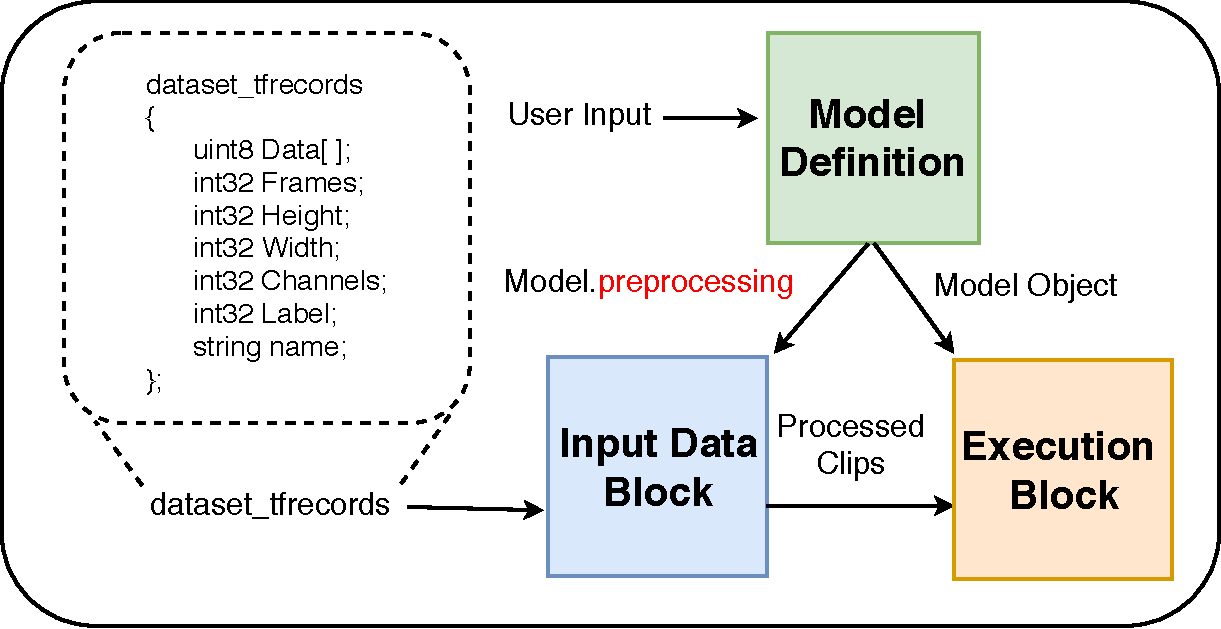
\includegraphics[width=0.8\textwidth]{images/overview.pdf}
\caption{Illustration of the two main components of \acro}
\label{fig:overview}
\end{figure}

\acro~is comprised of two main components, 1) the data input block, and 2) the execution block, as shown in Fig.~\ref{fig:overview}. 
The pipeline contained within the data input block can be divided into three simple stages,
\begin{enumerate}
\item Read video data from disk
\item Extract the desired number of clips from a given video
\item Preprocess the frames of clips using a selected model's preprocessing strategy.
\end{enumerate}
The execution block houses all of the code required to setup, train, test as well as log the outputs of a chosen model.
This includes defining the layers that comprise the model, training the model up to a predetermined number of epochs, saving parameter values of a model are regular intervals and finally testing the performance of the trained model over a variety of recognition metrics.
The following sections provide an in depth discussion of the setup and structure of various components of the platform.

\section{Input Pipeline}
\label{sec:ippipeline}
Included in the input pipeline are all of the steps required to pass a video into a model in the proper format.
The three stages of the input pipeline are detailed below.

\subsection{Read video data}
\label{sec:readdata}
When a training or testing instance is run on a model, the first step is to setup the tensorflow graph.
The first node in this graph is the tensorflow tfrecords file reader. 
Video data, stored as tfrecords, are read into the system in a FIFO queue.


\subsection{Extract clips}
\label{sec:extractclips}
Certain models, for example C3D~\ref{}, require their inputs to be in the form of multiple clips extracted from a single video.
To allow for the loading of multiple clips for each loaded video, another FIFO queue is added to the pipeline to store individual clips.
Fig.~\ref{fig:extract_clips} details the data flow from the tfrecords video data queue, through the clip extraction algorithm, and into the clips queue.
By default, the clip extraction algorithm is set to process and entire video at a time and only extract clips if the required arguments have been specified.

\begin{figure}[b!]
\centering
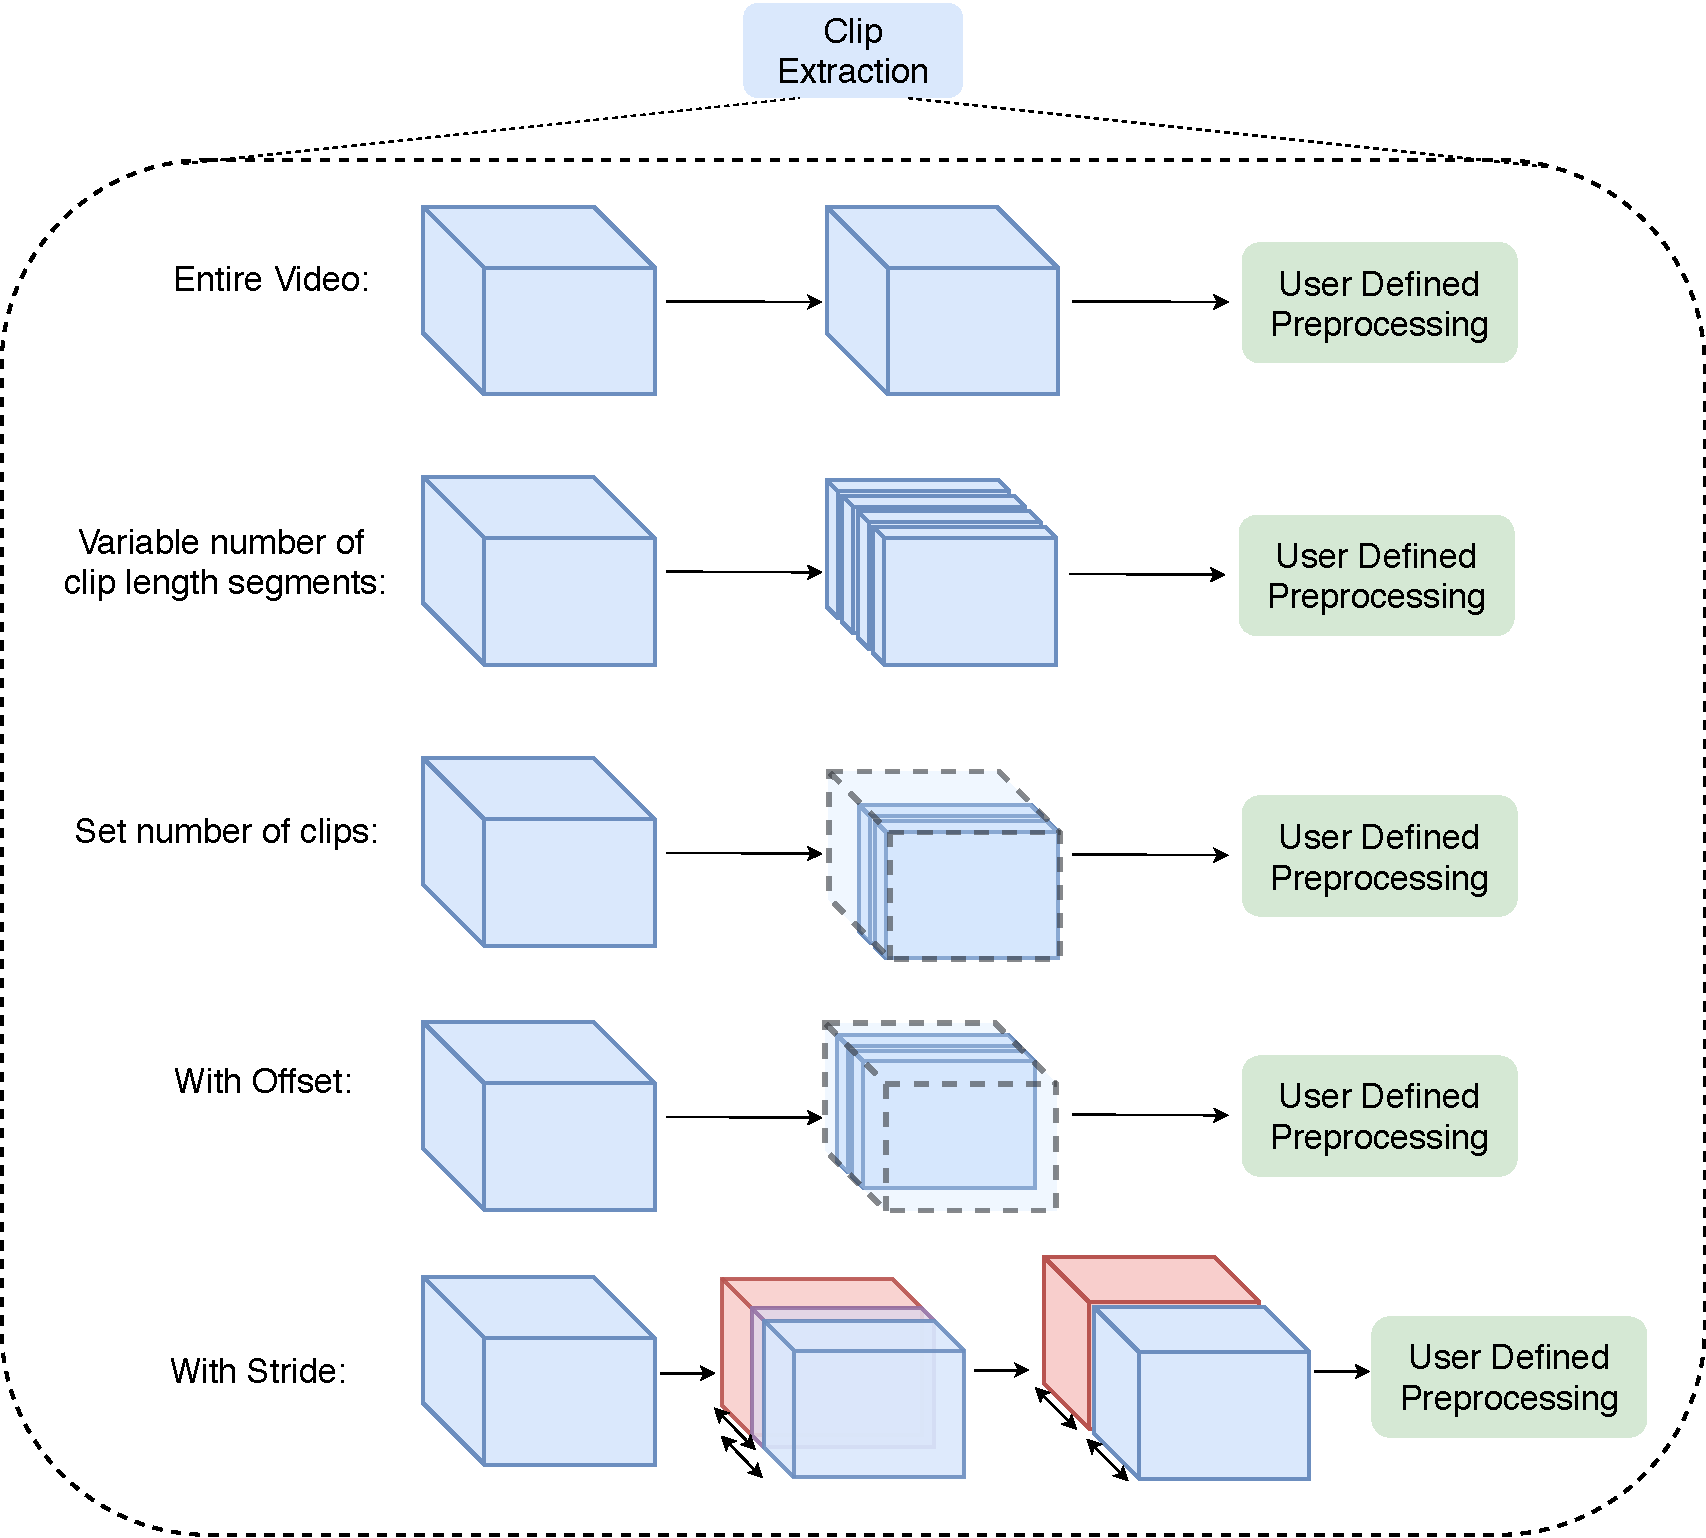
\includegraphics[width=0.8\columnwidth]{images/extract_clips.pdf}
\caption{The input pipeline allows for videos to be broken into clips according to defined specifications.
Whenever a video has been completely processed and used for training or testing, a new video is loaded from the queue.
The video is then passed through our clip extraction algorithm which enqueues the clips individually into a secondary queue.
Clips are then dequeued from the clips queue according to the number of GPUs being used and the required clip batch size.}
\label{fig:extract_clips}
\end{figure}


\subsection{Preprocess clips}
\label{sec:preprocessclips}
Activity recognition employ a number of various preprocessing methods on a frame or clip-based level.
These can include frame-wise cropping, flipping, and resizing, or clip-wise temporal offsets, resampling, and looping.
In order to incorporate these methods as desired per model, we create one or multiple preprocessing files for each model.
The desired preprocessing file for a model can be defined within the model and then called from the inputs call 

\acro~includes implementations of all of these options which can easily be added to a model's preprocessing file.



\section{Execution Block}
\label{sec:execblock}
Training and testing form the two main tenants of the execution block. 
Fig.~\ref{fig:exec_block} illustrates this partition along with the largest submodules present within each part.
Details regarding the flow of data and processes between various submodules and the entire execution block are provided below.

\begin{figure}[t!]
\centering
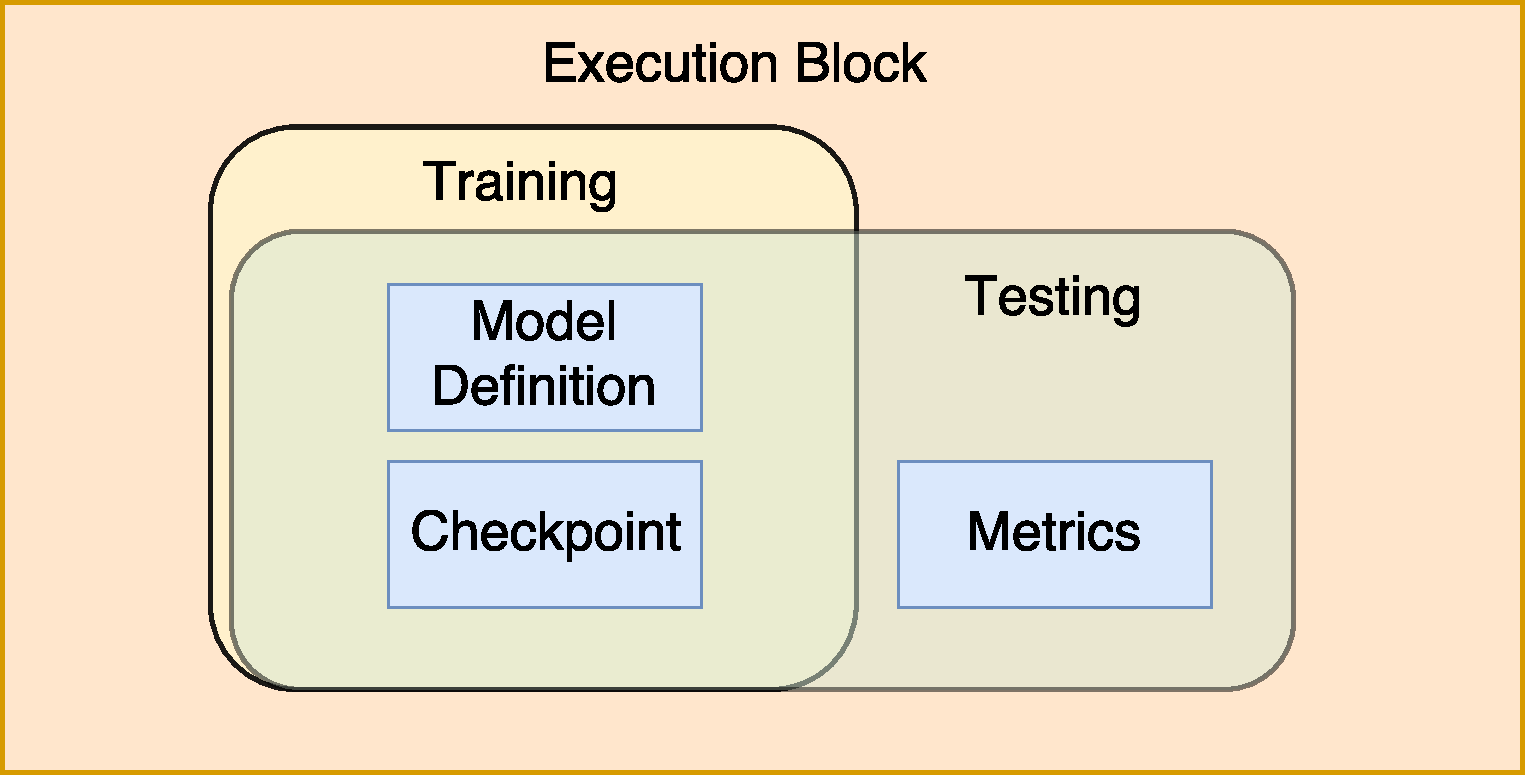
\includegraphics[width=0.8\columnwidth]{images/exec_block.pdf}
\caption{Training and Testing functions are the two major phases within the execution block. Model definitions and checkpoint-based functions are part of both training and testing functions while metrics are calculated after models are tested.}
\label{fig:exec_block}
\end{figure}

\subsection{Training: Algorithmic flow of processes}
\label{sec:training}
Training, within the context of the execution block, follows the process flow outlined in Alg.~\ref{}.
The beginning of every training experiment is aligned with a chosen model. 
Here, basic model parameters such as input/output data dimensions, batch normalization, dropout rate, and etc. are passed into the \model~in order to select and setup a desired model according to well defined prerequisites.

Once the model has been set up, the next step is to ensure that the parameter weights for the chosen model are retrieved. 
If the model has been pre-trained using \acro~and the user desires to further fine-tune the model, then the model parameter's weights from the latest checkpoint will be restored.
By default, the standard pre-trained weights, such as Kinetics~\cite{} for I3D~\cite{}, Sports1M~\cite{} for C3D~\cite{}, ImageNet~\cite{} for ResNet50~\cite{} and TSN~\cite{} are loaded into the model.
Alternatively, a random initialization option, for users to train from scratch is also provided. \\
Note: To ensure that there is a backup when a specified checkpoint is unavailable, the random intialization option is used, with the system providing a warning to the user about the setup used in training.

After the preparation of the model is complete, data tensors are retrieved from the \data.
The main data retuned from \data~are the video frames, their corresponding labels and video names.
With the availability of the model and data, the next stage is creating a copy of the model on the selected number of GPUs within a compute node.
\acro~only supports the extension of a model within a compute node of a cluster. 
Currently, it cannot be distrbute a model across mutiple nodes or split a model across multiple GPUs within a node.

Within each GPU, the inference function of \model~is used to generate a copy of the layer definitions. 
Here, the variable names are re-used to ensure that the same copy of weights are associated throughout all the GPUs.
From each of the model copies, we retrieve a desired layer's output. 
Given that the most common approach to training a network is through the use of logits returned from the final layer, we use the variable logits associated with the last layer to obtain a loss value.
Gradient computation based on the loss calculated is also performed.
Finally, the loss and gradients across all the model copies are accumulated into the loss\_array and gradients\_array respectively.
The contribution of each model copy is weights equally and the final gradient used to update the weights of the model is obtained by taking the average of value stored in the gradients\_array.
The is the final stage in the definition of the tensorflow graph required for training.

\begin{algorithmic}[H]
\Procedure{Training}{}
\State \textbf{Model\_definition}.\textcolor{red}{setup}(model\_params)
\State \textbf{Checkpoint}.\textcolor{red}{load\_param\_weights}(default or specific file)
\State Data, Labels = \textbf{DIB}.\textcolor{red}{load\_data}(expt\_params)
\\
\For{each GPU within given node}
\State \textbf{Model\_definition}.\textcolor{red}{inference}(Data, model\_params)
\State tower\_loss = \textbf{Model\_definition}.\textcolor{red}{loss}(Labels, returned\_logits)
\State tower\_gradients = gradients(tower\_loss)
\State loss\_array.store(tower\_loss)
\State gradients\_array.store(tower\_gradients)
\EndFor
\\
\State grad = average\_gradients(gradients\_array)
\State train\_op = apply\_gradients(grad)
\\
\While{no\_videos\_loaded \textless~(total\_epochs $\times$ videos\_in\_dataset)}
\State \textbf{Checkpoint}.\textcolor{red}{save}() @ regular intervals
\State sess.run(train\_op)
\State update(no\_videos\_loaded)
\EndWhile
\EndProcedure
\end{algorithmic}

After the tensorflow graph for training has been defined, the next step is to execute the graph. 
Usually, models are trained for a typical number of epochs, iterations over the entire dataset.
Within each epoch, based on a set frequency of iterations, we save the model parameter's weights using the save function within \checkpoint.
The main operation that gets executed within each iteration is the train\_op.
It is important to note that during the setup of th experiment, \acro~does not offsr adaptive learning rate control. Instead, two alternative arguments are used to specify fixed epoch boundaries at which the learning rate can decay and the scaling factor by which it does.

\subsection{Model Description Submodule}
\label{sec:modeldesc}
\begin{figure}[b!]
\centering
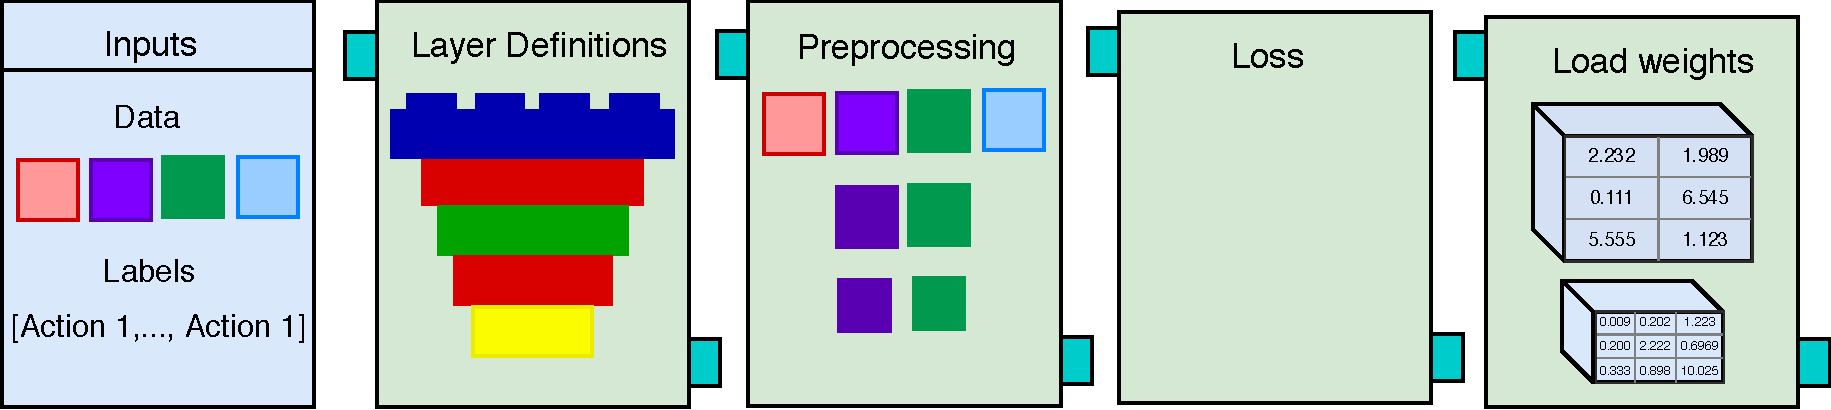
\includegraphics[width=\columnwidth]{images/model_submodule.pdf}
\caption{}
\label{fig:model_submodule}
\end{figure}

The class definition of a model within \acro~can be divided into four main components as shown in Fig.~\ref{}. 
The first step to incorporating a model in \acro~is to define the network architecture within an \textcolor{red}{inference} function.
The layers used must strictly be called from within the set of definitions provided within the \textcolor{blue}{layer\_utils} file.
This ensures that layer definitions are not specific to any network and become available to all models defined within \acro.
Further, it is essential that the inference function returns the outcome of any and all desired layers from within the defined network.
Any accompanying functions to help quickly and/or recursively define a network can be added outisde of the inference function.

Once the network has been defined, the next step is to setup the network's desired preprocessing formulation.
Concrete definitions of each preprocessing step can be included in a separate file.
We provide a standard list of preprocessing functions within the \textcolor{blue}{preprocessing\_utils} file that can be used to construct the entire preprocessing pipeline.
The expected output from a preprocessing function is the preprocessed input data.
Multiple preprocessing pipelines can be included within the same model with the use of the simple \textit{if-else} construct to quickly expand a model's abilities. 
Within the model definition file, it is sufficient to import and call a preprocessing method defined in the adjacent file.

In \acro, we attach the definition of any loss to a model to avoid cluttering and increasing the complexity of the main training file.
Thus, a basic loss function needs to be defined within a models class, with the expected return being logits.
However, the basic loss function can altenratively be used to call different loss functions by using the internally defined \texttt{\textcolor{ForestGreen}{loss\_type}} keyword.

The final and optional component of any model definition within \acro~is the definition of \textcolor{red}{load\_default\_weights} function.
This function is defined to ensure that a predetermined set of weights can be loaded onto the network defined.
The explicit rules required to define the layer names and ensure their respective weights can be assigned are provided in Section~\ref{sec:checkpoint}.
The final values returned by this function are the parameter weights loaded from an external file. 

In order to quickly define and integrate any model into \acro's pipeline, we provide a template file named \textcolor{blue}{models\_abstract.py} which provides the outline for the user to quickly fill out the inference, preprocessing, loss and load weights functions.
A separate file named \textcolor{blue}{models\_preprocessing\_template.py} provides a template for defining the preprocessing pipeline.

Note: 1) Any model defined must be placed within the models folder under a directory with the same name as that of the model,
2) No explicit model class attributes can be added to a specific model. Instead, they must be added to the model\_abstract.py file and made available to any and all model definitions within \acro.
The models that come standard with \acro~include the state-of-the-art activity recognition architectures I3D~\cite{}, C3D~\cite{}, ResNet50~\cite{}, and TSN~\cite{}.

\subsection{Checkpoint Submodule}
\label{sec:checkpoint}

\subsection{Testing: Flowchart of processes}
\label{sec:testing}

\subsection{Metrics Submodule}
\label{sec:metrics}

\section{Benchmarks}
\label{sec:benchmarks}

\clearpage

\bibliographystyle{splncs}
\bibliography{egbib}

\end{document}

\grid
\grid
\grid
\grid
\grid


